\begin{document}
\maketitle
\vspace{-0.8cm}

\begin{center}
\fcolorbox{blue!50!black}{blue!4}{\parbox{0.96\textwidth}{\small
\textbf{Resumen.} B3 (64$\times$384$\times$384) con la tesela por defecto de 16$\times$15 funciona a unos 4,5 GOPs, porque la
mayoría de las repeticiones caen en un ``estado lento'' en el que tanto el empaquetado como el cálculo van más despacio (\iss{48},
\iss{50}). Solo hemos cambiado el empaquetador de B, activado con una opción. La disposición de Bc, el microkernel, el bloqueo y el
modelo de caché no cambian. Hay ocho órdenes de lectura (el actual y siete variantes), y todos escriben un Bc idéntico byte a byte.

\textbf{Resultado 1.} \key{El disparador es leer 4 bytes de cada columna de B en cada acceso.} Los tres empaquetadores que lo hacen
(incluido el de cargas escalares) se vuelven lentos en la mayoría de las celdas de 16$\times$8 y 16$\times$15, incluso sin cálculo
entre empaquetados. Ninguno de ellos se vuelve lento en B3 con 16$\times$6.

\textbf{Resultado 2.} Leer una columna cada vez (\texttt{col-g1}, \texttt{col-g1-m4}) \key{no da ninguna repetición lenta en ninguna celda
GEMM, con ninguna tesela, K, placa o noche.} Con la tesela por defecto, \key{B3 pasa de 4,53--4,63 a 7,01--7,05 GOPs por tiempo medio} (de
4,28 a 7,00--7,05 por repetición mediana). B2 se queda a menos de 0,09 GOPs con \texttt{col-g1-m4} (0,21 con \texttt{col-g1}), y
Reuse24 ya no tiene repeticiones lentas.

\textbf{Resultado 3.} Leer 2, 4 o todas las columnas a la vez elimina el disparador de 4 bytes, pero vuelve a producir celdas malas
que dependen de la tesela y de K, no del tamaño del grupo. También aparece un estado nuevo, ``lento de forma estable''
(\texttt{col-g2} con K=256).}}
\end{center}

\noindent\textit{Los puntos clave van en} \key{negrita azul oscuro}\textit{.}

\paragraph{Cómo se tomaron los números.} Todas las velocidades vienen de la versión sin instrumentar (\texttt{INSTRUMENTED=0}),
protocolo de referencia, \texttt{-{}-tmin 10}, núcleo 4, \texttt{-{}-no-nc-overrides}, 3 lanzamientos por caso, rotación a la
izquierda, en la placa \texttt{jbpi2}. Una repetición (\emph{rep}) es una ejecución de la llamada cronometrada. La velocidad se da en
GOPs, por tiempo medio (la fórmula de la referencia) y por repetición mediana; ``\% lento'' es la proporción de repeticiones en
estado lento. La segunda placa, \texttt{jbpi}, se usó en la serie 1 solo como comprobación cruzada. No se leyeron contadores de la
placa.

\section{Contexto}
B está almacenada por columnas (\emph{column-major}). Bc contiene paneles de NR columnas, por filas dentro de cada panel: el elemento
$(k,j)$ del panel $p$ está en \texttt{Bc[p*NR*kc + k*NR + j]}. El empaquetador xDSL actual hace, para cada k, una carga con salto
\texttt{vlse32} que recoge 8 columnas. Con K=384 el salto es $\texttt{ldb}\cdot 4 = 1536$ B (\texttt{ldb} = 384 números entre el
inicio de dos columnas, por 4 bytes por número fp32), así que \key{cada instrucción toca 8 líneas de caché y toma 4 B de cada una.}

Lo que encontraron los issues anteriores: el estado lento sigue a NR (\iss{48}); el empaquetador escalar es más estable pero no más
barato (\iss{53}); rellenar \texttt{ldb} cambia el estado, pero no de forma sencilla (\iss{49}); y las repeticiones lentas reducen
a la mitad los aciertos de precarga de la L1D (\iss{50}). El X60 no tiene Zicbop y su precargador (\emph{prefetcher}) no está
documentado. Por eso este trabajo cambia el patrón de lectura que ve el precargador y observa el resultado.

\paragraph{Los tamaños que importan (Figura~\ref{fig:units}).} Un registro vectorial tiene VLEN\,=\,256 bits, así que contiene 8
valores fp32; RVV tiene 32 registros, y LMUL\,=\,4 une cuatro en un grupo de 128 B con 32 valores. La configuración \texttt{jbpi2} del
modelo de caché da una L1D de 32 KB (128 conjuntos $\times$ 4 vías $\times$ líneas de 64 B) y una L2 de 512 KB (1024 conjuntos
$\times$ 8 vías $\times$ 64 B). La B de B3 es 384$\times$384 fp32 = 576 KB; una columna ocupa 1536 B = 24 líneas, y una línea
contiene 16 valores de k consecutivos de una columna. El bloqueo en estas ejecuciones es mc\,=\,64, nc\,=\,384, y kc\,=\,256 con
16$\times$6 y 16$\times$8, 128 con 16$\times$15 (según los ficheros por repetición). Así, un bloque Bc ocupa 384 KB con 16$\times$6 y
16$\times$8 (64 o 48 paneles) y 195 KB con 16$\times$15 (26 paneles de 15$\times$128 valores = 7,5 KB cada uno): siempre más que la
L1D y dentro de la L2.

\paragraph{Cómo leer los números 4 y 8.} Una carga del empaquetador actual llena un registro vectorial con 8 números; cada número es
un valor fp32 de 4 bytes, y cada uno viene de una columna distinta de B. Así que una carga toma 4 B de cada una de 8 columnas, 32 B
en total, de 8 líneas de caché distintas. En las figuras, ``8'' siempre cuenta números, columnas o líneas de caché, nunca bytes.

\paragraph{Los distintos 4 del código.} El número 4 aparece en el código con dos significados distintos, que se confunden con
facilidad:
\begin{center}\footnotesize\setlength{\tabcolsep}{5pt}
\begin{tabular}{@{}lp{11.2cm}@{}}
\toprule
dónde & qué significa el 4 \\
\midrule
\texttt{ldb * 4} (carga del empaquetador actual) & 4 \textbf{bytes} por número fp32. \texttt{ldb} cuenta números (384 en B3), y la
instrucción quiere el salto en bytes: $384 \times 4 = 1536$ B entre dos números de una carga. No significa ``4 elementos'': la carga
sigue leyendo 8 números. \\
\texttt{RR * 4} (escritura de la solución) & también 4 bytes por número: una fila del panel Bc tiene NR números, así que la fila
siguiente empieza $\mathrm{NR} \times 4$ bytes después (60 B con NR\,=\,15). \\
\texttt{m4}, LMUL\,=\,4 (carga de la solución) & 4 \textbf{registros vectoriales} unidos en un registro largo. Un registro contiene
8 números, así que cuatro contienen 32: una carga lee 32 números. \\
``4 B de cada columna'' (en el texto) & un número fp32 ocupa 4 bytes. \\
\bottomrule
\end{tabular}
\end{center}

\begin{figure}[!htb]
\centering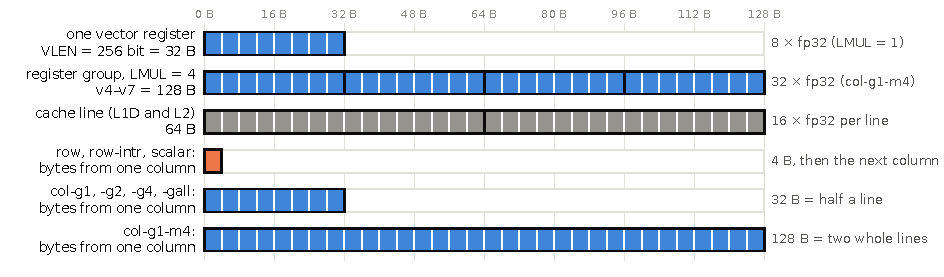
\includegraphics[width=\textwidth]{fig_units.pdf}
\figcap{Tamaños de registro, de línea de caché y de cada acceso, dibujados a la misma escala de bytes. Una celda es un fp32 (4 B).
Las tres filas de abajo muestran lo que toma un acceso a una columna de B con cada orden de lectura (propiedad C).}
\label{fig:units}
\end{figure}

\section{Las tres propiedades y las variantes}
Un orden de lectura tiene tres propiedades: (A) cómo se emite una lectura (vectorial con salto, escalar o vectorial contigua); (B)
cuántas columnas se leen a la vez; (C) cuántos bytes se toman de una columna en cada acceso. Cada variante cambia estas propiedades, y
solo estas. Todas las variantes escriben el mismo Bc: una prueba en el ordenador anfitrión las compara byte a byte, y la prueba en
la placa (5400 casos) da 0 errores. \texttt{col-gall} lee hasta 24 columnas a la vez; aquí NR es como máximo 24, así que equivale a NR.

\begin{center}\footnotesize\setlength{\tabcolsep}{4pt}
\begin{tabular}{@{}lp{5.4cm}lcc@{}}
\toprule
variante & cómo se lee B & A: emisión & B: columnas a la vez & C: bytes por columna \\
\midrule
\texttt{row} (actual, xDSL) & \texttt{vlse32} a través de 8 columnas por k & vectorial con salto & NR & 4 \\
\texttt{row-intr} & lo mismo, escrito con intrínsecos de C & vectorial con salto & NR & 4 \\
\texttt{scalar} & un elemento cada vez & escalar & NR & 4 \\
\texttt{col-gall} & \texttt{vle32} de 8 valores bajando por cada columna, las NR columnas a la vez, y luego escrituras con salto en Bc & vectorial contigua & NR & 32 \\
\texttt{col-g4} & lo mismo, 4 columnas a la vez & vectorial contigua & 4 & 32 \\
\texttt{col-g2} & lo mismo, 2 columnas a la vez & vectorial contigua & 2 & 32 \\
\texttt{col-g1} & una columna cada vez (el orden que pedía \iss{44}) & vectorial contigua & 1 & 32 \\
\texttt{col-g1-m4} & una columna cada vez, LMUL\,=\,4: 32 valores por carga & vectorial contigua & 1 & 128 (dos líneas enteras) \\
\bottomrule
\end{tabular}
\end{center}
\texttt{row-intr} es un control: debería comportarse como \texttt{row}. Si no lo hace, es que el propio camino en C cambia algo (véase
Limitaciones).

\paragraph{La solución, y por qué no puede cambiar el resultado (Figura~\ref{fig:fixflow}).} Un empaquetador solo copia números; no
hace ninguna operación aritmética. Todos los órdenes de lectura ponen cada número de B en el mismo sitio de Bc,
\texttt{Bc[k*NR + j] = B(k, j)}; solo cambia el orden de las copias. El empaquetador actual carga una fila de B (8 números, uno por
columna) en un registro y la escribe como una fila de Bc. La solución carga 32 números de una columna en cuatro registros unidos
(LMUL\,=\,4) y los escribe bajando por una columna de Bc. Cuando el panel está terminado, \key{los dos Bc son idénticos byte a byte}, así
que el microkernel recibe la misma entrada, hace las mismas operaciones en el mismo orden y da la misma C, bit a bit. Esto se ha
comprobado, no solo razonado:
\begin{itemize}
  \item \textbf{Disposición, en el anfitrión:} \texttt{test\_pack\_b\_variants.py} compara cada variante con el empaquetador escalar
  byte a byte (NR de 1 a 31, paneles parciales, restos de kc, \texttt{ldb} > kc, huecos de relleno sin tocar). Un error introducido a
  propósito (la tira de 32 números sin cortar al final de una columna) hizo fallar la prueba.
  \item \textbf{Disposición, en la placa} (\texttt{jbpi2}, GCC 13.2, \texttt{-O2} y \texttt{-O3}): la misma prueba con el código RVV
  real, 5400 casos (6 variantes $\times$ 10 NR $\times$ 5 kc $\times$ 6 nc $\times$ 3 \texttt{ldb}), 0 errores.
  \item \textbf{GEMM completa, en la placa:} cada una de las 6 variantes con 16$\times$15, en B3 y B3\_K256, con el resultado
  comprobado frente a la referencia: 12 de 12 correctas (PASS).
  \item \textbf{Cada ejecución de solo empaquetado de las dos series} repite el empaquetado con el empaquetador escalar y compara todo
  el Bc: 108 de 108 ejecuciones \texttt{ok}.
\end{itemize}
Una limitación: las ejecuciones GEMM cronometradas de las Tablas 1--4 no comprueban el resultado (eso frenaría el bucle de
medida); su corrección se apoya en las comprobaciones anteriores.

\paragraph{Por qué la solución no hace más lento nada más.} Cambiar el orden de lectura podría, en principio, costar velocidad en tres
sitios. \key{En ninguno se ve una pérdida.}
\begin{itemize}
  \item \textbf{El microkernel.} Lee Bc, no B, y Bc es idéntico byte a byte y está en el mismo sitio. Así que el microkernel hace las
  mismas cargas y las mismas operaciones que antes. La solución solo cambia el paso de empaquetado y, a través de él, si la ejecución
  cae en el estado lento (que frena tanto el empaquetado como el cálculo, \iss{50}).
  \item \textbf{Las escrituras dispersas en Bc.} La solución cambia lecturas dispersas de B por escrituras dispersas en Bc (un número
  cada 60 B con 16$\times$15). Este es el lado más barato: todas las escrituras caen dentro del panel que se está llenando, 7,5 KB con
  16$\times$15 (120 líneas), que cabe de sobra en la L1D de 32 KB, así que las 15 pasadas por columnas vuelven a líneas que muy
  probablemente siguen en la L1. Las lecturas de B, en cambio, vienen de una matriz de 576 KB que no está en la L1. Coste medido: un
  empaquetado rápido tarda 0,8218 ms frente a 0,6443 ms de \texttt{row-intr} (16$\times$15, B3, Tabla 3). Pero la solución nunca se
  vuelve lenta, así que su empaquetado medio es más barato: 0,822 ms frente a 1,155 ms (Figura~\ref{fig:packcost}).
  \item \textbf{Formas que nunca eran lentas.} B2 y Reuse24 no tienen estado lento que eliminar, así que solo muestran el lado del
  coste. B2 se queda a menos de 0,09 GOPs de \texttt{row} con \texttt{col-g1-m4} (Tabla 4), dentro de la variación entre ejecuciones.
  Reuse24 queda igual o algo mejor con 16$\times$6 y 16$\times$8 (9,29 frente a 9,21; 9,15 frente a 8,95), y mejor con 16$\times$15
  (8,87 frente a 8,48), donde \texttt{row} tiene un 14--17\% de repeticiones lentas. En B3 con 16$\times$6, donde \texttt{row} tampoco
  es nunca lento, la solución es algo más rápida (6,89 frente a 6,72 GOPs).
\end{itemize}
La razón ``aciertos en la L1 al escribir'' es la más probable, no una medida: estas ejecuciones no leyeron contadores.

\begin{figure}[!htb]
\centering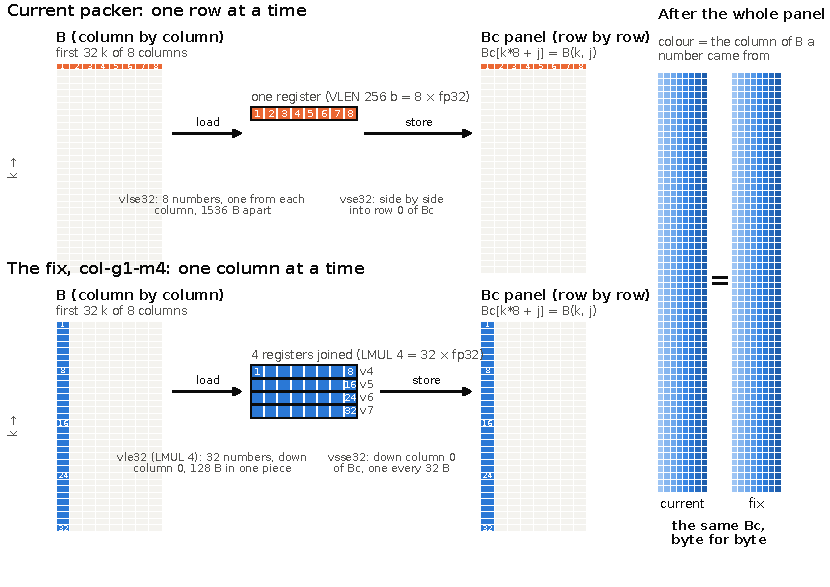
\includegraphics[width=\textwidth]{fig_fix_dataflow.pdf}
\figcap{Una carga y una escritura del empaquetador actual (arriba) y de la solución (abajo), de B a través del registro o registros
vectoriales hasta Bc; dibujado para NR\,=\,8 y los primeros 32 valores de k de un panel. Los números indican por qué posición del
registro pasa cada valor. A la derecha: el panel terminado, con cada número coloreado según la columna de B de la que viene: igual en
los dos casos.}
\label{fig:fixflow}
\end{figure}

\paragraph{La solución en el código C (Figura~\ref{fig:codediff}).} La solución cambia tres sitios del empaquetador y nada más:
\textbf{(1)} el orden de los bucles, de ``k fuera, columnas dentro'' a ``columna fuera, k dentro''; \textbf{(2)} la carga, de una
\texttt{vlse32} con salto de 8 números (salto \texttt{ldb*4} = 1536 B) a una \texttt{vle32} contigua de 32 números (LMUL\,=\,4);
\textbf{(3)} la escritura, de una \texttt{vse32} contigua en una fila de Bc a una \texttt{vsse32} con salto bajando por una columna de
Bc (salto \texttt{RR*4}). El destino de cada número, \texttt{Bp + i*RR + c} frente a \texttt{Bp + i*RR + jj}, es el mismo elemento de
Bc. Nota sobre los 4: en \texttt{ldb*4} y \texttt{RR*4} el 4 es el tamaño de un número fp32 en bytes (los intrínsecos reciben los
saltos en bytes), así que \texttt{ldb*4} = 384 números $\times$ 4 B = 1536 B; no es un número de elementos. En \texttt{m4}
(LMUL\,=\,4) el 4 es el número de registros vectoriales unidos: 4 registros de 8 números = 32 números por carga.

\begin{figure}[!htb]
\centering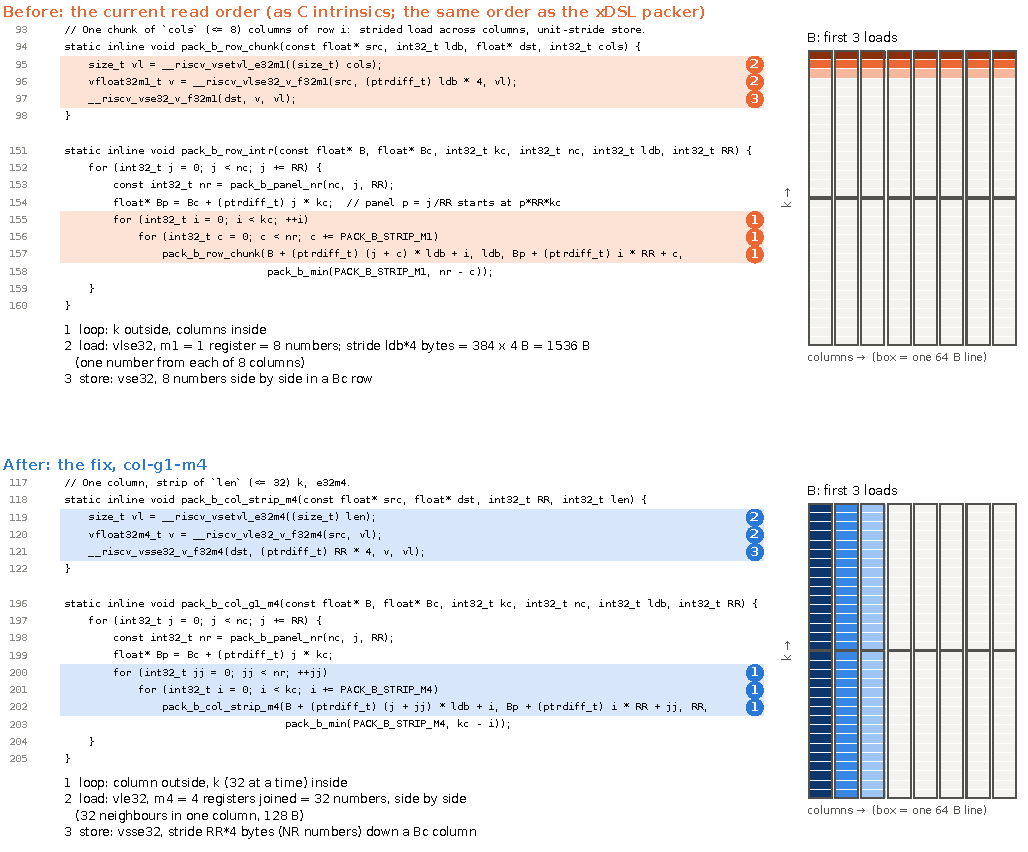
\includegraphics[width=\textwidth]{fig_code_diff.pdf}
\figcap{Antes y después, en intrínsecos de C, copiado literalmente de
\texttt{tests/pure\_xdsl\_blis\_rvv/templates/pack\_b\_variants.h} (números de línea a la izquierda). ``Antes'' es el orden de lectura
actual escrito en C (\texttt{row-intr}, el mismo bucle que el empaquetador xDSL del Apéndice~C.2--C.3); ``después'' es la solución.
Las líneas marcadas son los tres cambios: 1 el orden de los bucles, 2 la carga, 3 la escritura. En \texttt{ldb * 4} y
\texttt{RR * 4} el 4 son bytes por número fp32 (un salto en bytes); en \texttt{m4} son 4 registros unidos (32 números). A la derecha:
las tres primeras cargas que emite cada versión sobre B (oscura, media, clara), para 8 columnas y 32 valores de k; cada recuadro es
una línea de caché de 64 B.}
\label{fig:codediff}
\end{figure}

\paragraph{Qué pide cada orden a la memoria (Figuras~\ref{fig:order} y~\ref{fig:counts}).} Contado a partir de los bucles, para un
panel completo de B3 con la tesela por defecto (NR\,=\,15, kc\,=\,128: 1920 valores, 7,5 KB, 120 líneas de B). El orden actual emite
256 cargas con salto (8\,+\,7 valores por k); cada una toca 7 u 8 líneas de B y toma 4 B de cada una, así que las 15 columnas están
abiertas a la vez y cada línea de B se visita 16 veces, una por cada k. \texttt{col-g1-m4} emite 60 cargas; cada una toma dos líneas
enteras de una columna, así que solo hay una columna abierta cada vez y cada línea de B se visita una sola vez. El coste pasa al lado
de las escrituras: una escritura con salto de \texttt{col-g1-m4} reparte sus 32 valores en 30 líneas de Bc (salto de 60 B), frente a
1--2 líneas de la escritura contigua de \texttt{row}. Las ejecuciones de la \S\ref{sec:packonly} muestran que este intercambio
compensa.

\begin{figure}[!htb]
\centering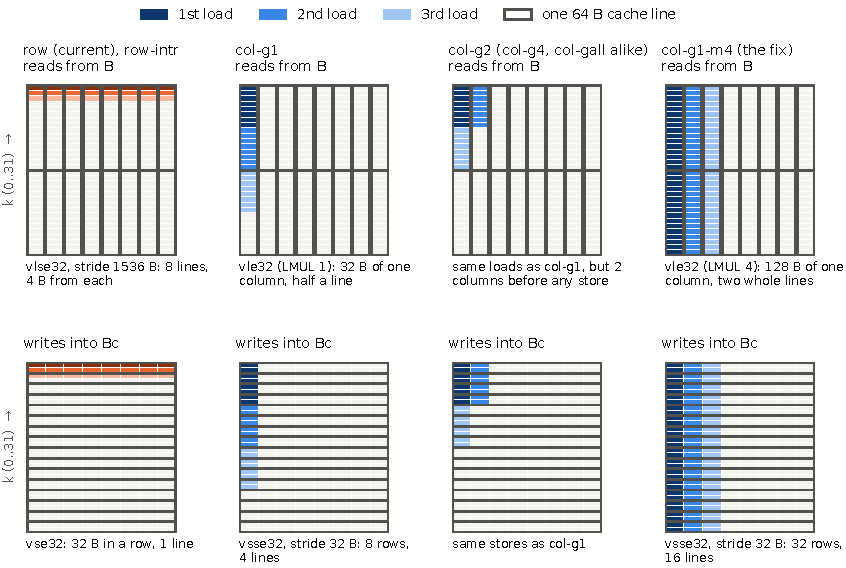
\includegraphics[width=0.9\textwidth]{fig_read_order.pdf}
\figcap{Las tres primeras cargas de cada orden de lectura (oscura, media, clara) y dónde acaban en Bc. Dibujado para NR\,=\,8 (la
tesela 16$\times$8, una \texttt{vlse32} por k) y los primeros 32 valores de k de un panel; \texttt{row} aparece en naranja. Arriba: B
está almacenada por columnas, así que cada columna es contigua y cada recuadro es una línea de 64 B (16 valores de k). Abajo: el panel
Bc está almacenado por filas; una fila de 8 valores ocupa 32 B y una línea contiene dos filas. \texttt{row} cruza 8 líneas por carga
para tomar un valor de cada una; los órdenes por columnas leen bajando por una columna y escriben a través de las filas.}
\label{fig:order}
\end{figure}

\begin{figure}[!htb]
\centering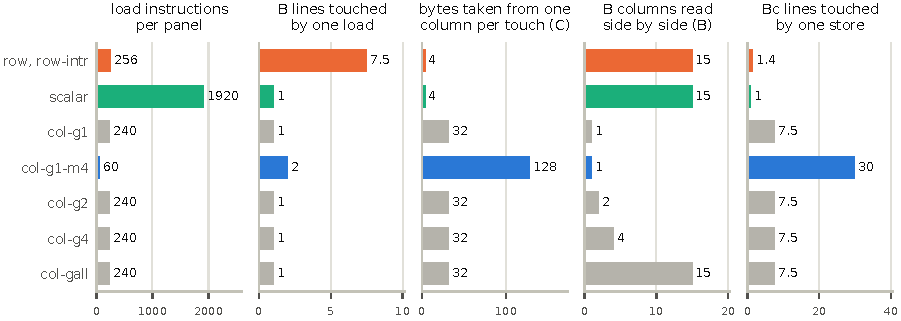
\includegraphics[width=\textwidth]{fig_counts.pdf}
\figcap{Un panel completo de B con la tesela por defecto (B3, NR\,=\,15, kc\,=\,128, ldb\,=\,384), contado repitiendo los bucles de
los empaquetadores (\texttt{issue-54-figs/make\_figs.py}, \texttt{panel\_instructions}), con líneas de 64 B y B y Bc alineadas a línea.
No está medido en la placa. Naranja: el orden actual; azul: la solución; verde: escalar.}
\label{fig:counts}
\end{figure}

\section{Resultados: B3 y B3\_K256}
Cada celda es GOPs por tiempo medio / GOPs por repetición mediana / \% lento. Se fijan tres teselas (16$\times$6, 16$\times$8,
16$\times$15), cada una con B3 (K=384) y B3\_K256. S1 es la serie 1 y S2 la serie 2. \texttt{row}, \texttt{col-g1-m4} y
\texttt{col-gall} se ejecutaron en las dos; \texttt{row-intr}, \texttt{scalar} y \texttt{col-g1} solo en S1; \texttt{col-g2} y
\texttt{col-g4} solo en S2. En rojo y negrita: celdas malas (alguna repetición lenta, o lentas de forma estable).
La Figura~\ref{fig:headline}(a) muestra juntos el empaquetador actual, \texttt{scalar} y la solución; la Figura~\ref{fig:heatmap}
muestra todas las celdas.

\begin{figure}[!htb]
\centering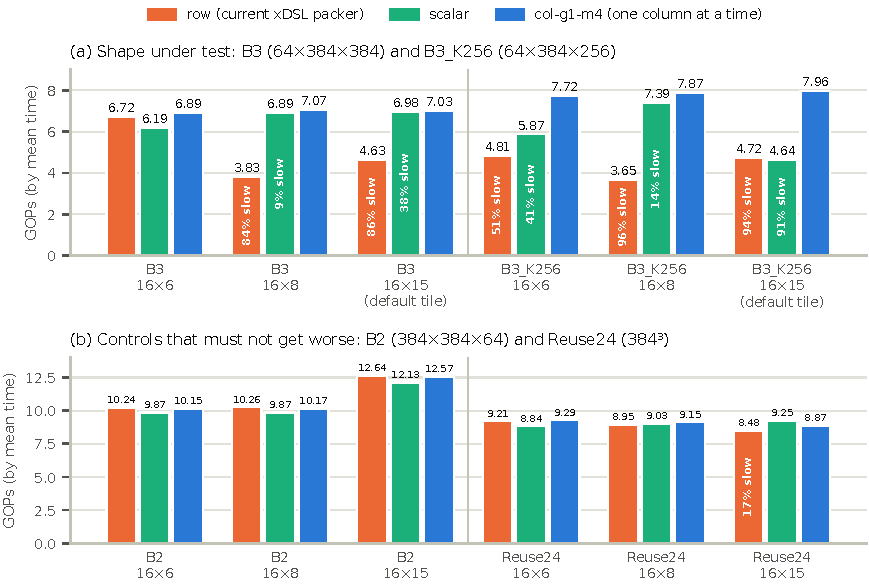
\includegraphics[width=0.9\textwidth]{fig_headline.pdf}
\figcap{Serie 1 en \texttt{jbpi2}: \texttt{row}, \texttt{scalar} y \texttt{col-g1-m4} se ejecutaron la misma noche. La altura de la
barra son los GOPs por tiempo medio en 3 lanzamientos; la etiqueta blanca dentro de la barra es su proporción de repeticiones lentas.
Sin instrumentar (\texttt{INSTRUMENTED=0}), protocolo de referencia \texttt{-{}-tmin 10}, núcleo 4, \texttt{-{}-no-nc-overrides}.
Fuente: \texttt{report\_series1\_jbpi2.md}, sección 1.}
\label{fig:headline}
\end{figure}

\begin{figure}[!htb]
\centering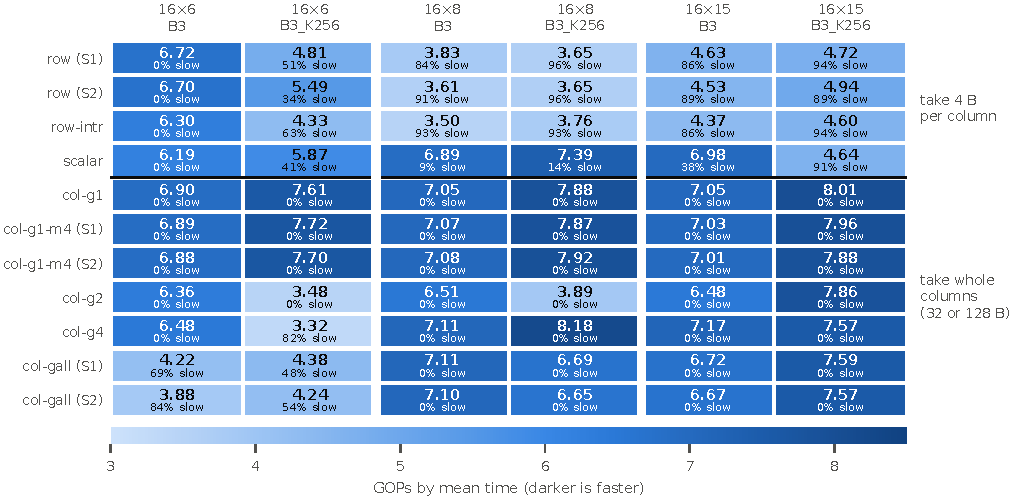
\includegraphics[width=0.9\textwidth]{fig_heatmap.pdf}
\figcap{Todas las celdas GEMM de las Tablas 1 y 2: GOPs por tiempo medio (en negrita) y proporción de repeticiones lentas. Más oscuro
es más rápido. Por encima de la línea negra, los órdenes que toman 4 B por columna; por debajo, los que toman columnas enteras. Una
celda clara con ``0\% slow'' (\texttt{col-g2} con K\,=\,256) es el estado lento de forma estable de la \S\ref{sec:insight}. Misma
versión, protocolo y placa que la Figura~\ref{fig:headline}; fuentes: los dos informes de serie, sección 1.}
\label{fig:heatmap}
\end{figure}

\paragraph{Lectores que toman 4 bytes por columna.}
\begin{center}\footnotesize\setlength{\tabcolsep}{2.8pt}
%%TAB3%%
\end{center}
{\footnotesize Tabla 1. Sin instrumentar (INSTRUMENTED=0), protocolo de referencia \texttt{-{}-tmin 10}, núcleo 4,
\texttt{-{}-no-nc-overrides}, 3 lanzamientos, placa \texttt{jbpi2}. Fuente: \texttt{report\_series1\_jbpi2.md} y
\texttt{report\_series2\_jbpi2.md}, sección 1.}

\paragraph{Lectores que toman columnas enteras.}
\begin{center}\footnotesize\setlength{\tabcolsep}{2.8pt}
%%TAB4%%
\end{center}
{\footnotesize Tabla 2. Sin instrumentar (INSTRUMENTED=0), protocolo de referencia \texttt{-{}-tmin 10}, núcleo 4,
\texttt{-{}-no-nc-overrides}, 3 lanzamientos, placa \texttt{jbpi2}. Fuente: los mismos dos informes, sección 1. En verde: ninguna
repetición lenta y en línea con los demás lectores por columnas.}

Los dos lectores \texttt{col-g1} no tienen ninguna repetición lenta en ninguna de sus 18 celdas, y las celdas S1 y S2 de
\texttt{col-g1-m4} coinciden con una diferencia de menos de 0,08 GOPs. Las dos celdas de \texttt{col-g2} con K=256 en 16$\times$6 y
16$\times$8 tampoco tienen repeticiones lentas, pero van a 3,48 y 3,89 GOPs, frente a 7,70 y 7,92 de \texttt{col-g1-m4} (detalles en
la \S\ref{sec:insight}).

\emph{Comprobación cruzada en \texttt{jbpi}} (solo serie 1): todas las celdas GEMM caen en la misma clase, lentas o estables. Las
celdas estables de \texttt{col-g1} y \texttt{col-g1-m4} quedan a menos de 0,15 GOPs de \texttt{jbpi2}, y las celdas en estado lento
varían hasta 0,43 GOPs.

\clearpage
\section{Resultados: el bucle de solo empaquetado}
\label{sec:packonly}
Este bucle ejecuta el empaquetador de B solo, sin cálculo entre empaquetados y con una lectura del reloj por repetición. Cada celda es
proporción de repeticiones lentas (\%) / tiempo medio de las repeticiones rápidas (ms). Cuando un empaquetador es casi siempre lento,
su media ``rápida'' se calcula sobre pocas repeticiones.

\begin{center}\footnotesize\setlength{\tabcolsep}{4pt}
%%TAB5%%
\end{center}
{\footnotesize Tabla 3. Sin instrumentar (INSTRUMENTED=0), protocolo de referencia \texttt{-{}-tmin 10}, núcleo 4,
\texttt{-{}-no-nc-overrides}, 3 lanzamientos, placa \texttt{jbpi2}. Fuente: \texttt{report\_series1\_jbpi2.md} y
\texttt{report\_series2\_jbpi2.md}, sección 2. \texttt{row} y 16$\times$6 no están en este bucle.}

Con lecturas de 4 bytes, el empaquetador solo ya muestra dos velocidades: \texttt{row-intr} es lento en un 91\% con 16$\times$15 y con
16$\times$8 en B3, y \texttt{scalar} en un 84--95\% con 16$\times$15. Los lectores por columnas se quedan en un 0--7\%. El 4--7\% de
repeticiones lentas de \texttt{col-g1} y \texttt{col-g1-m4} con 16$\times$8 son repeticiones aisladas (por ejemplo, 0,5598 ms rápida
frente a 0,7851 ms lenta para \texttt{col-g1-m4} en B3), y no aparecen en las celdas GEMM.

\paragraph{Las dos velocidades, repetición a repetición (Figura~\ref{fig:reps}).} Con el orden actual, la GEMM es rápida en sus
primeras 18 repeticiones, se vuelve lenta a los 0,05 s y se queda en una franja cercana a 4,3 GOPs (mediana de las repeticiones
lentas: 4,33), con vueltas cortas a la velocidad rápida; el empaquetador de B solo hace lo mismo, de unos 0,6 ms a unos 1,3 ms por
repetición. Con \texttt{col-g1-m4}, los dos se quedan en una sola franja durante toda la ejecución.

\paragraph{Coste medio por empaquetado (Figura~\ref{fig:packcost}).} Contando todas las repeticiones, también las lentas, un
empaquetado de B3 tarda 0,822 ms con \texttt{col-g1-m4} frente a 1,155 ms con \texttt{row-intr} con 16$\times$15, y 0,574 ms frente
a 1,147 ms con 16$\times$8. Una repetición rápida de \texttt{row-intr} es más barata (la marca negra), pero es poco frecuente.
\texttt{row} no está en este bucle, así que la comparación es con su copia en intrínsecos de C.

\begin{figure}[!htb]
\centering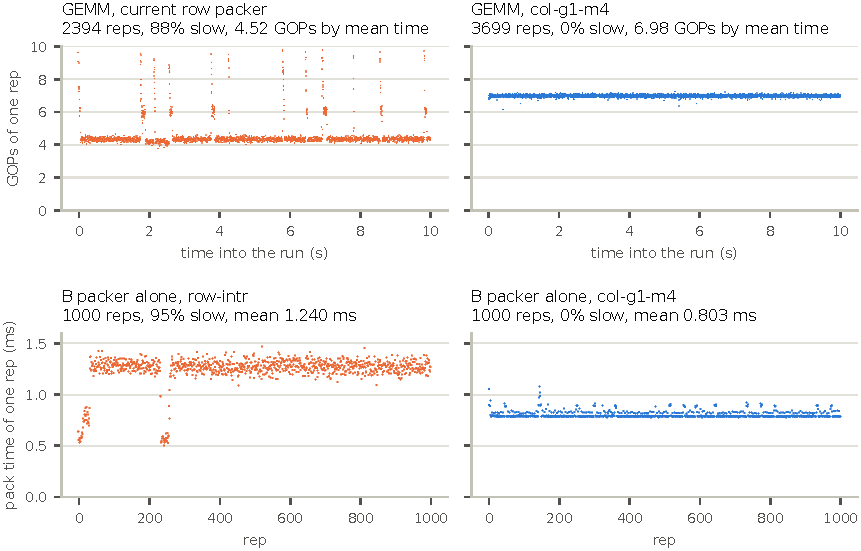
\includegraphics[width=\textwidth]{fig_reps.pdf}
\figcap{Todas las repeticiones de un lanzamiento, B3 con la tesela por defecto 16$\times$15. Arriba: la GEMM completa, serie 2,
lanzamiento 1 (\texttt{row}: \texttt{run\_2026-10-23\_101023}; \texttt{col-g1-m4}: \texttt{run\_2026-10-23\_103733}), un punto por
repetición frente al tiempo transcurrido en la ejecución de 10 s. Abajo: el empaquetador de B solo, serie 1, lanzamiento 1
(\texttt{packonly\_jbpi2\_L1\_*\_B3\_16x15.txt}), 1000 repeticiones tras 5 de calentamiento. Las proporciones lentas usan la misma
separación que los informes de serie. Son lanzamientos únicos, así que las proporciones difieren un poco de las medias de 3
lanzamientos de las Tablas 1 y 3. Sin instrumentar, protocolo de referencia \texttt{-{}-tmin 10}, núcleo 4,
\texttt{-{}-no-nc-overrides}, \texttt{jbpi2}.}
\label{fig:reps}
\end{figure}

\begin{figure}[!htb]
\centering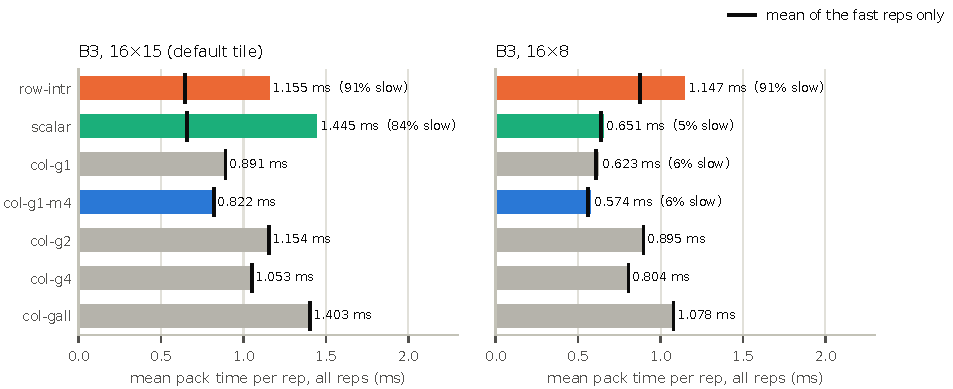
\includegraphics[width=\textwidth]{fig_pack_cost.pdf}
\figcap{El empaquetador de B solo, en B3. Barra: tiempo medio por repetición sobre todas las repeticiones, media de 3 lanzamientos;
marca negra: la media de las repeticiones rápidas solamente (el valor de la Tabla 3). \texttt{col-g2} y \texttt{col-g4} son de la
serie 2, el resto de la serie 1. Sin instrumentar, núcleo 4, \texttt{jbpi2}; fuente: los ficheros \texttt{packonly\_jbpi2\_L*} de las
dos series.}
\label{fig:packcost}
\end{figure}

\section{Resultados: los controles B2 y Reuse24}
GOPs medios; entre paréntesis, la proporción de repeticiones lentas cuando no es cero (la serie 1 aparece en la
Figura~\ref{fig:headline}(b)). B2 usa kc$=$64; Reuse24 usa el mismo kc que B3 con cada tesela (256, 256, 128).

\begin{center}\footnotesize\setlength{\tabcolsep}{4pt}
%%TAB6%%
\end{center}
{\footnotesize Tabla 4. Sin instrumentar (INSTRUMENTED=0), protocolo de referencia \texttt{-{}-tmin 10}, núcleo 4,
\texttt{-{}-no-nc-overrides}, 3 lanzamientos, placa \texttt{jbpi2}. Fuente: los dos informes, sección 1 (bloques B2 y R24).}

En B2 los lectores por columnas quedan a menos de 0,26 GOPs de \texttt{row} (la mayor diferencia es 12,64 frente a 12,38,
\texttt{col-gall} S1, con 16$\times$15; \texttt{col-g1-m4} como mucho 0,09); \texttt{scalar} es entre 0,37 y 0,51 más bajo. Reuse24
solo se vuelve lento con \texttt{row} (16$\times$15: 17\% en S1, 14\% en S2) y con \texttt{row-intr} (16$\times$8: 73\%;
16$\times$15: 53\%). Ningún lector por columnas se vuelve lento en ninguno de los dos controles.

\section{Qué significa para el diseño}
\label{sec:insight}
\begin{enumerate}
  \item \textbf{Es un patrón de lectura lo que provoca el estado lento; no la unidad vectorial ni el número de flujos.} Lo que tienen
  en común \texttt{row}, \texttt{row-intr} y \texttt{scalar} es que toman 4 B de cada una de NR columnas separadas 1536 B (B3) o
  1024 B (B3\_K256), y luego pasan al siguiente k. Las cargas escalares también lo hacen: el solo empaquetado es lento en un 84--95\%
  con 16$\times$15, y la GEMM completa en un 91\% con 16$\times$15 en B3\_K256. Así que el resultado de \iss{53} de que ``el escalar
  es más estable'' depende de la tesela.
  \item \textbf{El empaquetador de B por sí solo puede provocar el estado.} En el bucle de solo empaquetado, sin cálculo,
  \texttt{row-intr} es lento en un 91\% con 16$\times$15 y con 16$\times$8 en B3. Así que el siguiente paso corresponde al
  empaquetador, no al orden entre empaquetado y cálculo.
  \item \textbf{Leer una columna 32 B o 128 B cada vez elimina este disparador.} \key{Una columna cada vez es el único orden seguro en todas
  las celdas que probamos.}
  \item \textbf{Agrupar columnas vuelve a producir celdas malas, que dependen de la tesela y de K, no del tamaño del grupo.}
  \texttt{col-g2} es malo con K=256 (16$\times$8 y 16$\times$6), \texttt{col-g4} es malo con 16$\times$6 y K=256, y \texttt{col-gall}
  es malo con 16$\times$6 con las dos K. Esto parece un efecto de colocación (dónde caen en la caché las líneas activas), lo que
  encaja con \iss{49}, y no un límite en el número de flujos. La idea de \iss{44} es correcta en su efecto (una columna cada vez), pero
  por otro motivo.
  \item \textbf{Un tercer estado: lento de forma estable.} \texttt{col-g2} con 16$\times$8 en B3\_K256 va a 3,89 GOPs con una
  variación entre lanzamientos de 0,02 (3,88--3,90) y sin división en dos velocidades. Su empaquetado solo tarda de forma uniforme
  0,6448 ms (mediana), frente a 0,2500 ms de \texttt{col-g1-m4}. Una herramienta que separa las repeticiones en rápidas y lentas marca
  esta celda como 0\% lenta. Hay que leer los GOPs junto con la proporción lenta.
  \item \textbf{Coste.} En una repetición rápida, el empaquetado por columnas cuesta algo más que el de \texttt{row-intr}: con
  16$\times$15 en B3, la media rápida del solo empaquetado es 0,8218 ms para \texttt{col-g1-m4} frente a 0,6443 ms. Pero nunca se
  vuelve lento, mientras que \texttt{row-intr} pasa el 91\% de sus repeticiones en 1,1994 ms.
  \item \textbf{El fallo está en el método de empaquetado habitual, no solo en este diseño: la referencia también lo tiene.} El diseño
  de referencia (\texttt{gemm\_blis\_family} en \texttt{RVV\_ukernels\_benchmark}) empaqueta B en el mismo orden: la lectura del código
  de \iss{52} encontró que su empaquetador de B visita las mismas direcciones en el mismo orden que el nuestro, 4 B de cada columna a
  lo largo de una fila, solo que con una carga escalar por elemento. Y cae en el mismo estado lento en B3\_K256 (\iss{46}, más abajo).
  En B3 normal, la referencia era mucho más estable que la nuestra en \iss{46}, pero no en la nueva ejecución de más abajo (81\% lenta
  con 16$\times$14); el motivo no está claro. Las razones más probables son su tesela (16$\times$14 frente a nuestra 16$\times$15) y
  dónde caen sus búferes: el parche de medida por repetición movió su velocidad en B3 en direcciones opuestas en las dos placas. Como
  lee B de la misma forma, el empaquetador por columnas debería ayudar también a la referencia, y la nueva ejecución de más abajo lo
  confirma (16$\times$14: 4,49 $\to$ 7,14 GOPs). El código exacto de los dos empaquetadores está en el Apéndice~C.

  La Figura~\ref{fig:refvsours} muestra las lecturas de los dos empaquetadores y de la solución, sobre la matriz y sobre las direcciones
  de memoria.

  \begin{figure}[!htb]
  \centering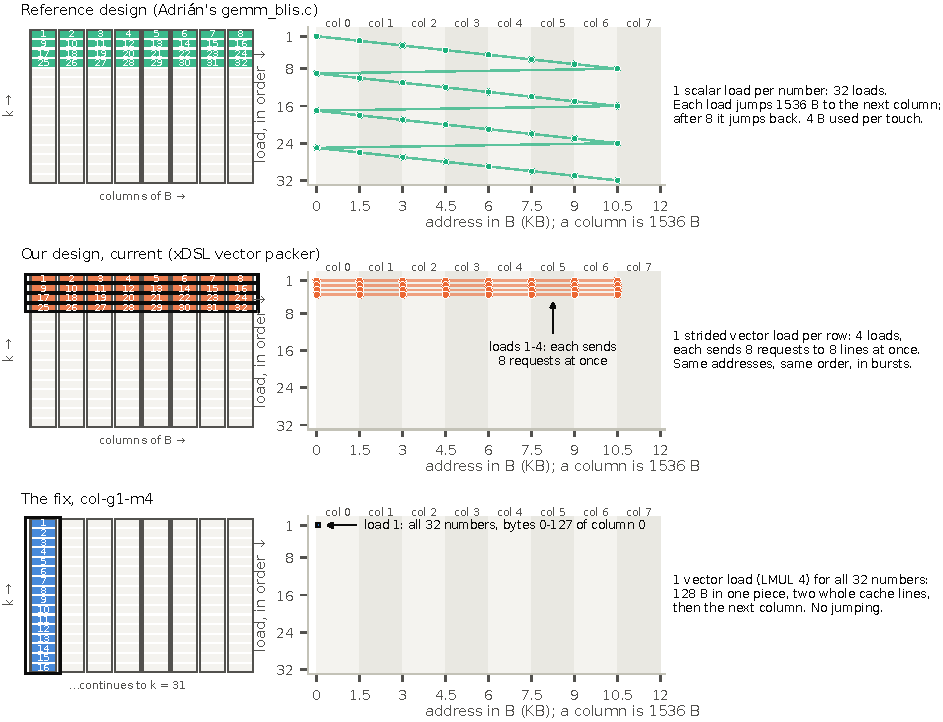
\includegraphics[width=\textwidth]{fig_ref_vs_ours.pdf}
  \figcap{Los primeros 32 números que cada empaquetador lee de la B de B3 (K\,=\,384, así que las columnas están separadas 1536 B).
  Izquierda: sobre la matriz, numerados en orden de lectura; una línea de caché es una columna recuadrada de 16 números. Derecha: las
  mismas lecturas sobre las direcciones de memoria de B, una fila por instrucción de carga. La referencia (\texttt{pack\_CB} en
  \texttt{gemm\_blis.c}) y el empaquetador xDSL actual leen los mismos números en el mismo orden: 4 B de la columna 0, luego 1536 B
  más allá para la columna 1, y así sucesivamente, volviendo a la columna 0 después de 8. La referencia emite una carga por número; el
  nuestro emite una carga vectorial con salto por fila, así que las mismas 8 peticiones dispersas salen a la vez. La solución lee 32
  números bajando por una columna con una sola carga. Dibujado a partir del código, NR\,=\,8; con NR\,=\,15 la vuelta atrás llega
  después de 15 columnas.}
  \label{fig:refvsours}
  \end{figure}

  \begin{center}\footnotesize\setlength{\tabcolsep}{5pt}
  \begin{tabular}{@{}lcc@{}}
  \toprule
  repeticiones lentas (\texttt{jbpi} / \texttt{jbpi2}) & nuestro, 16$\times$15, empaquetador vectorial & referencia, 16$\times$14 \\
  \midrule
  B3\_K256 & \bad{94\% / 88\%} & \bad{80\% / 60\%} \\
  B3 & \bad{87--89\%}, 4,4--4,5 GOPs & \bad{22\%} / 0\%, 7,1--7,6 GOPs \\
  \bottomrule
  \end{tabular}
  \end{center}
  {\footnotesize Tabla 5. De \iss{46} (2026-09-29, una serie más antigua que el resto de este informe, ejecutada en momentos tranquilos
  en las dos placas): sin instrumentar, protocolo de referencia \texttt{-{}-tmin 10}, núcleo 4; el programa de prueba de la referencia
  solo se modificó para registrar el tiempo de cada repetición. No es la misma noche que las Tablas 1--4, así que solo se debe comparar
  dentro de esta tabla.}

  \textbf{Nueva ejecución: el diseño de referencia con nuestra solución (2026-10-29).} El diseño de referencia de Adrián se volvió a
  ejecutar en B3, tal cual y con su \texttt{pack\_CB} sustituido por nuestro empaquetador por columnas
  (\texttt{ref\_baseline/ref\_pack\_fix.py}, en una copia preparada; nada más cambió; la comprobación del resultado pasa con error 0 en
  las dos teselas). Con 16$\times$14, la referencia tal cual era lenta en un \bad{81\%}, 4,49 GOPs (4,39--4,60 en 3 lanzamientos); \key{con
  la solución no tuvo ninguna repetición lenta, 7,14 GOPs (7,11--7,18), +59\%.} Con 16$\times$16, un kernel que es más lento por sus
  propios motivos (necesita 34 registros vectoriales, \iss{46}), la solución lo lleva de 4,20 a 4,41 GOPs y de un 22\% a un 0\% de
  repeticiones lentas (Figuras~\ref{fig:refcompare} y~\ref{fig:refreps}). Esto difiere de \iss{46}, donde la B3 de la referencia con
  16$\times$14 era lenta en un 0--22\%. Aquella ejecución medía cuatro formas en un mismo binario y esta mide solo B3, y \iss{46}
  encontró que la velocidad de la referencia en B3 cambia según dónde caen sus búferes; así que la referencia no es de forma fiable más
  estable en B3 que nuestro diseño. \key{La solución elimina el estado lento en los dos diseños.}

  \begin{figure}[!htb]
  \centering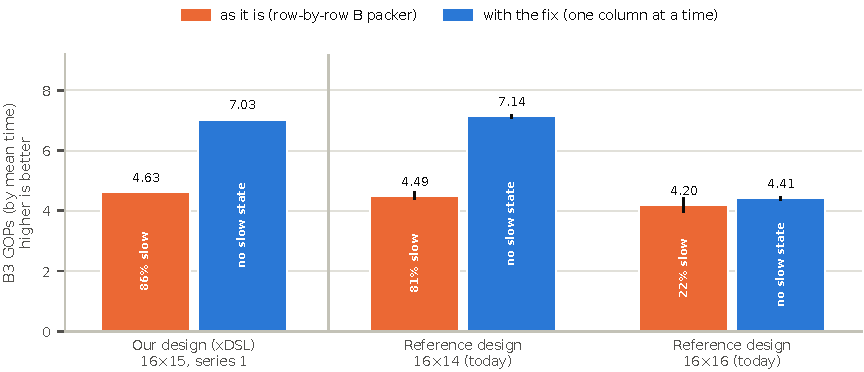
\includegraphics[width=0.92\textwidth]{fig_ref_compare.pdf}
  \figcap{B3 con y sin la solución, en nuestro diseño y en el diseño de referencia. Barra: GOPs por tiempo medio, media de 3
  lanzamientos; línea fina: del lanzamiento más bajo al más alto; texto en la barra: proporción de repeticiones lentas. Nuestro
  diseño: serie 1 (2026-10-22, Tabla 1). Diseño de referencia: 2026-10-29, con el programa, los empaquetadores y los kernels LDX
  \texttt{macc} de la propia referencia, y el registro por repetición; la referencia no tiene kernel de 16$\times$15, así que se
  ejecutan sus vecinos 16$\times$14 y 16$\times$16. Noches distintas: compárese dentro de cada diseño, no entre diseños. Todo sin
  instrumentar, protocolo de referencia \texttt{-{}-tmin 10}, núcleo 4, placa \texttt{jbpi2}, orden de lanzamientos A B, B A, A B; la
  placa estaba libre al 98,6--99,5\% y sin otros usuarios antes y después de cada ejecución. Carpetas: serie
  \texttt{logs/issue54\_ref\_2026-10-29\_123319} (\texttt{runs.tsv}; referencia \texttt{refbase\_2026-10-29\_123934},
  \texttt{\_125611}, \texttt{\_130140}; con la solución \texttt{refbase\_2026-10-29\_124512}, \texttt{\_125042}, \texttt{\_130709}).}
  \label{fig:refcompare}
  \end{figure}

  \begin{figure}[!htb]
  \centering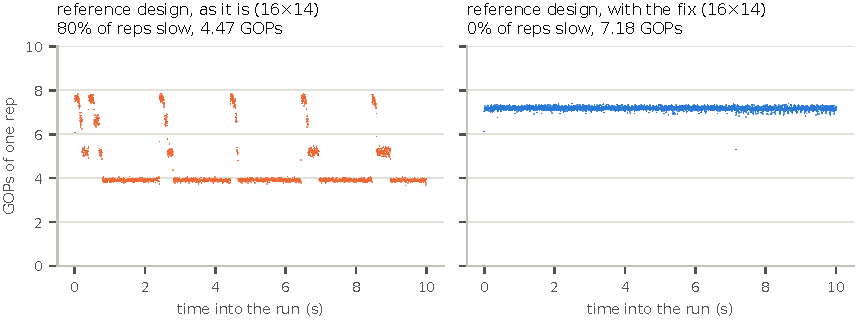
\includegraphics[width=\textwidth]{fig_ref_reps.pdf}
  \figcap{Todas las repeticiones del lanzamiento 1, B3, el diseño de referencia con 16$\times$14: tal cual (izquierda,
  \texttt{refbase\_2026-10-29\_123934}) y con nuestra solución en su empaquetador (derecha, \texttt{refbase\_2026-10-29\_124512}). Las
  mismas dos velocidades que en nuestro diseño (Figura~\ref{fig:reps}); con la solución, una sola velocidad. Misma versión, protocolo,
  núcleo y placa que la Figura~\ref{fig:refcompare}.}
  \label{fig:refreps}
  \end{figure}

  \item \textbf{Nuestro empaquetador vectorial hace más frecuente el estado lento en la mayoría de las celdas, pero no lo causa.} Misma
  noche y misma placa (Tabla 1, serie 1), proporción de repeticiones lentas, \texttt{row} vectorial frente a \texttt{scalar}: 84\%
  frente a 9\% con 16$\times$8 en B3, 96\% frente a 14\% con 16$\times$8 en B3\_K256, 86\% frente a 38\% con 16$\times$15 en B3, 51\%
  frente a 41\% con 16$\times$6 en B3\_K256. Pero con 16$\times$15 en B3\_K256 los dos son lentos (94\% y 91\%), con 16$\times$6 en B3
  ninguno lo es, y en el bucle de solo empaquetado el orden se invierte con 16$\times$15 en B3\_K256 (\texttt{row-intr} 33\%,
  \texttt{scalar} 95\%, Tabla 3). Cuando ninguno es lento, el empaquetador vectorial es el más rápido (6,72 frente a 6,19 GOPs con
  16$\times$6 en B3). Una razón probable, no medida: una carga vectorial con salto envía 8 peticiones a 8 líneas distintas a la vez,
  mientras que el empaquetador escalar envía las mismas 8 una a una, así que el patrón malo llega en ráfagas. Por tanto, la causa es el
  patrón de lectura, que comparten el vectorial, el escalar y la referencia. El empaquetador vectorial lo empeora en la mayoría de las
  celdas. Volver al escalar no lo arregla, y los vectores no son el problema: la solución usa cargas vectoriales aún más anchas (32
  números en lugar de 8), dirigidas hacia abajo por una columna en lugar de a lo largo de una fila.
  \item \textbf{Qué dice el desarrollador de la referencia, y qué muestran el código y los datos.} La opinión del desarrollador de la
  referencia (2026-10-29): el empaquetado y el desempaquetado en sí no tienen ningún fallo evidente; el salto de direcciones al leer B
  es inofensivo en su empaquetador escalar, que lee un elemento cada vez, y se convierte en un problema cuando ese bucle se ensancha a
  código vectorial. El código máquina coincide (Apéndice~C.6): el empaquetador de la referencia, compilado con
  \texttt{-O3 -march=rv64gcvzfh}, no tiene ninguna instrucción vectorial, solo un par \texttt{flw}/\texttt{fsw} por número, separados
  1536 B; el nuestro convierte el mismo bucle en cargas \texttt{vlse32.v} que envían 8 (luego 7) peticiones a otras tantas columnas a la
  vez. Los datos también coinciden en gran parte:
  \begin{itemize}
    \item En B3 la referencia escalar es lenta en un 0--22\%, la nuestra en un 87--89\% (Tabla 5); nuestro propio empaquetador escalar
    es lento en un 9--14\% con 16$\times$8 frente a un 84--96\% del vectorial, y en un 38\% frente a un 86\% con 16$\times$15 en B3
    (Tabla 1). Así que, en estas ejecuciones, ensanchar el bucle hace que nuestro diseño caiga en el estado lento mucho más a menudo.
    \item Pero la nueva ejecución del 2026-10-29 (Figura~\ref{fig:refcompare}) encontró la referencia escalar lenta en un 81\% en B3
    con 16$\times$14, y nuestra solución también lo eliminó allí (4,49 $\to$ 7,14 GOPs). Así que leer un número por carga no mantiene
    B3 estable en todas las ejecuciones.
  \end{itemize}
  Con un límite: el orden fila a fila tampoco está del todo libre del problema con cargas escalares. La referencia sigue siendo lenta
  en un 60--80\% en B3\_K256 (Tabla 5), nuestro empaquetador escalar es lento en un 91\% con 16$\times$15 en B3\_K256 (Tabla 1), y
  solo, en un 84--95\% con 16$\times$15 (Tabla 3). Así que la afirmación precisa es: el empaquetado es correcto y su orden fila a fila
  es casi siempre inofensivo con cargas escalares; ensancharlo a cargas vectoriales con salto hace el estado lento mucho más
  frecuente; y con K\,=\,256 el orden tiene un coste incluso con cargas escalares. La solución mantiene el ancho vectorial y cambia la
  dirección de las lecturas, así que evita las dos cosas (Tablas 1--2). B solo se empaqueta, nunca se desempaqueta, en la GEMM, así
  que el desempaquetado no influye aquí.
\end{enumerate}

\section{¿Merece la pena la solución? Comparación con las opciones más sencillas}
\label{sec:worth}
Hay dos opciones más sencillas que no necesitan código nuevo: activar el empaquetador escalar de B que el generador ya tiene (su
opción es \texttt{use\_scalar\_pack}), o elegir una tesela más pequeña. La Tabla~6 compara el empaquetador actual, el escalar y la
solución en todas las capas y teselas, de la misma noche (serie 1).

\begin{center}\footnotesize\setlength{\tabcolsep}{4pt}
%%TAB8%%
\end{center}
{\footnotesize Tabla 6. GOPs por tiempo medio, 3 lanzamientos; entre paréntesis, la proporción de repeticiones lentas cuando no es
cero. Serie 1, la misma noche para los tres empaquetadores; sin instrumentar (\texttt{INSTRUMENTED=0}), protocolo de referencia
\texttt{-{}-tmin 10}, núcleo 4, \texttt{-{}-no-nc-overrides}, placa \texttt{jbpi2}. Fuente: \texttt{report\_series1\_jbpi2.md},
sección 1. Las pérdidas del 1\% de la solución en B2 están dentro de la variación entre ejecuciones.}

\paragraph{¿La mejora es grande?} Frente al empaquetador actual, sí, pero solo en la familia B3: \key{+52\% en B3 y +69\% en B3\_K256} con
la tesela por defecto, y hasta +116\% con 16$\times$8. En las capas grandes (B2, Reuse24) casi no cambia nada ($-$1\% a +5\%). Así
que es una mejora grande para un tipo de capas (M pequeña, K grande; \iss{35} encontró el estado lento hasta M\,=\,512 con la tesela
por defecto), no una aceleración de todo el diseño.

\paragraph{¿Por qué no quedarse simplemente con un empaquetador escalar?} En B3 normal con la tesela por defecto, el escalar es casi
igual de bueno (6,98 frente a 7,03 GOPs), no necesita código nuevo y es como empaqueta la referencia. Pero por sí solo no basta:
\begin{itemize}
  \item sigue cayendo en el estado lento en B3\_K256 con la tesela por defecto (91\% lento, 4,64 GOPs, frente a 7,96 de la solución), y
  con 16$\times$6 (41\%);
  \item cuando nada es lento, es más lento: $-$3 a $-$4\% en B2, la capa más grande (12,13 frente a 12,64 con 16$\times$15), y $-$8\%
  en B3 con 16$\times$6 (6,19 frente a 6,72);
  \item solo es mejor que la solución en una celda, Reuse24 con 16$\times$15 (9,25 frente a 8,87).
\end{itemize}
Así que el empaquetado escalar cambia una pérdida del 3--4\% en las capas grandes por un arreglo que funciona en B3 pero no en
B3\_K256. \key{La solución es la única de las tres que nunca es lenta y nunca es claramente más lenta}: la mejor o a menos de un 1\% en 11
de las 12 celdas.

\paragraph{¿Por qué no una tesela más pequeña?} 16$\times$6 mantiene B3 estable con el empaquetador actual (6,72 GOPs), pero no
B3\_K256 (51\% lento), y cuesta un 19\% en B2 (10,24 frente a 12,64). No es una solución.

\paragraph{¿Es una complicación innecesaria?} El cambio en sí es pequeño: 16 líneas de intrínsecos de C
(Figura~\ref{fig:codediff}), las mismas instrucciones que el empaquetador ya usa, dirigidas a leer bajando por las columnas. El coste
real es portarlo a xDSL: el dialecto todavía no tiene una escritura fp32 con salto (\iss{44}). Si ese coste compensa depende de algo
que no hemos medido: \textbf{cuánto tiempo de un modelo real se pasa en capas como B3} (M pequeña, K de 256 o más). Si esas capas son
raras, la opción escalar, o el empaquetador actual, es suficiente; si son frecuentes, la solución es la única opción de las
consideradas que elimina el estado lento en todos los casos.

\paragraph{¿Hace falta empaquetar?} Este trabajo no prueba una GEMM sin empaquetado; los dos diseños empaquetan, como hace BLIS, para
que el microkernel lea Bc en orden. La pregunta aquí es solo qué empaquetador usar, no si empaquetar o no.

\paragraph{Recomendación.} Antes de portarlo a xDSL, tomar la lista de capas de los modelos objetivo y contar el tiempo en capas con
M pequeña y K grande (trabajo de escritorio, a partir de las ejecuciones por capa que ya existen). \key{Portar la solución si esa
proporción es significativa;} si no, activar el empaquetador escalar solo para esas capas y aceptar la diferencia en B3\_K256.

\section{Limitaciones}
\begin{itemize}
  \item El control solo se cumple en parte. En las celdas de 16$\times$8 y 16$\times$15, \texttt{row-intr} queda a menos de 0,35 GOPs
  de \texttt{row}, con una proporción lenta parecida. Pero es más bajo en B3 con 16$\times$6 (6,30 frente a 6,72, S1), y en B3\_K256
  con 16$\times$6 la diferencia es mayor (4,33 frente a 4,81; 63\% frente a 51\% lento). También se vuelve lento en Reuse24 donde
  \texttt{row} no (16$\times$8). La copia en intrínsecos de C no es idéntica al empaquetador xDSL. Las mejoras de \texttt{col-g1} se
  mantienen frente a los dos.
  \item \texttt{col-g1-m4} existe solo en intrínsecos de C. Usarlo en el generador requiere portarlo a xDSL. Eso queda fuera del
  alcance de este trabajo, porque el dialecto no tiene una escritura fp32 con salto (\iss{44}).
  \item Solo formas de la familia B3 más dos controles, tres teselas fijas y un modelo de placa. En estas ejecuciones no se leyeron
  contadores (sin instrumentar), así que la explicación del precargador se deduce de \iss{50}; no se ha medido aquí.
  \item \textcolor{red}{NOTA ROJA, \texttt{jbpi} (solo placa de comprobación).} Una ejecución GEMM se descartó por la compilación de
  otro usuario, y una de solo empaquetado porque la inactividad total bajó al 84,8\%, por debajo del umbral del 85\%; las dos se
  repitieron. El núcleo 3 estuvo al 72\% durante un binario de 16$\times$15 de \texttt{run\_2026-10-22\_214815} (\texttt{col-g1-m4},
  lanzamiento 2), y el proceso de root \texttt{bluetoothd} usó entre un 20 y un 99\% de un núcleo en las lecturas de \texttt{top}
  (mediana 55\%). Los números de \texttt{jbpi} solo se usan como comprobación cruzada; todos los números de las tablas anteriores son
  de \texttt{jbpi2}.
  \item La proporción lenta de \texttt{row} cambia entre noches en algunas celdas (B3\_K256 con 16$\times$6: 51\% en S1, 34\% en S2).
\end{itemize}

\section{Próximos pasos}
\begin{itemize}
  \item Portar \texttt{col-g1-m4} a xDSL (nuevo ticket; necesita una escritura fp32 con salto, o el par carga contigua y escritura con
  salto).
  \item Una ejecución con contadores (al estilo de \iss{50}) de \texttt{row} frente a \texttt{col-g1-m4} en B3 con 16$\times$15, para
  confirmar la explicación del precargador.
  \item Estudiar las celdas malas de los lectores agrupados frente a las direcciones de Bc y de B (colocación). Es trabajo de
  escritorio y no necesita tiempo de placa.
  \item Arreglos del script de informes: marcar las celdas lentas de forma uniforme; una NOTA ROJA falsa por el \%CPU acumulado de
  \texttt{ps}; la carga durante la ejecución tomada del monitor por núcleo.
\end{itemize}

\section*{Apéndice A: fuentes}
\raggedright\emergencystretch=3em
\begin{itemize}
  \item Rama \texttt{issue55-pack-b-variants}: \texttt{5338a3b8} (variantes), \texttt{c85f7f7d} (opción), \texttt{d0de1b0f} (bucle de
  solo empaquetado, scripts de serie y de informe), \texttt{383c886c} (registros de la serie 1), \texttt{bf6f2366} (registros de la
  serie 2).
  \item Registros, en \path{tests/pure_xdsl_blis_rvv/}: \path{logs/issue55_2026-10-22_194043/report_series1_jbpi2.md};
  \path{logs/issue55_jbpi/issue55_2026-10-22_194043/report_series1_jbpi.md} (comprobación cruzada);
  \path{logs/issue55_2026-10-23_100122/report_series2_jbpi2.md}.
  \item Diseño de referencia con y sin la solución (2026-10-29): serie \path{logs/issue54_ref_2026-10-29_123319} y sus seis carpetas
  \path{refbase_2026-10-29_*}; código \path{ref_baseline/ref_pack_fix.py}, \path{run_issue54_ref.sh},
  \path{ref_baseline/cases_issue54_b3.tsv}.
  \item Figuras: \path{.scratch/reports/issue-54-figs/make_figs.py} genera todas las figuras a partir de los registros anteriores (se
  ejecuta desde la raíz del repositorio con el entorno virtual del proyecto). Las Figuras~\ref{fig:units}--\ref{fig:counts} están
  dibujadas y contadas a partir del código, no medidas.
  \item Issues \iss{54} (pregunta), \iss{55} (especificación), \iss{48}, \iss{49}, \iss{50}, \iss{53}, \iss{44}.
\end{itemize}

\clearpage
\section*{Apéndice B: el resultado en tres minutos}
\label{sec:short}
Una versión corta para una presentación, con palabras sencillas. Solo compara tres empaquetadores: el del diseño de referencia,
nuestro empaquetador xDSL actual y la solución. Cada paso indica la figura que se debe mostrar. Todas las velocidades vienen de la
versión sin instrumentar, protocolo de referencia, núcleo 4, placa \texttt{jbpi2}.

\newcommand{\step}[3]{\par\noindent\begin{minipage}{\textwidth}\textbf{#1}\par\smallskip #2\par\smallskip
\ifdim #3pt>0pt {\centering\includegraphics[width=#3\textwidth]{\stepfig}\par}\fi\end{minipage}\par\bigskip}

\def\stepfig{fig_short_reps.pdf}
\step{1. El problema: el estado lento.}{B3 es una capa de nuestra GEMM. Con la tesela por defecto debería ir a unos 7 GOPs, pero va a
unos 4,5. No es lenta todo el tiempo: empieza rápida y, tras 18 repeticiones (0,05 s), baja a una velocidad lenta y casi siempre se
queda ahí. Lo llamamos \emph{estado lento}. \key{Unas 9 de cada 10 repeticiones son lentas.} Izquierda: nuestro empaquetador actual;
derecha: la solución.}{0.9}

\def\stepfig{fig_ref_reps.pdf}
\step{1b. El mismo problema en el diseño de referencia (Figura~\ref{fig:refreps}).}{El diseño de referencia de Adrián, ejecutado en
la misma placa y de la misma forma (2026-10-29), muestra las mismas dos velocidades en B3 con su tesela más cercana, 16$\times$14:
rápida durante un momento y luego unos 3,9 GOPs, con un 81\% de repeticiones lentas. Con nuestra solución en su empaquetador, \key{se
mantiene en unos 7,1--7,2 GOPs sin ninguna repetición lenta.} Izquierda: la referencia tal cual; derecha: la referencia con la
solución.}{0.9}

\step{2. Lo que habíamos visto antes de este trabajo.}{%
\begin{itemize}
  \item En las repeticiones lentas el precargador del hardware trabaja la mitad de bien: trae por adelantado la mitad de líneas de
  caché (\iss{50}).
  \item El estado lento depende de cómo se empaqueta B, no de la parte de cálculo (\iss{48}).
  \item El empaquetador ejecutado solo, sin cálculo, también se vuelve lento.
\end{itemize}
Así que son las lecturas de memoria del empaquetador las que lo provocan.}{0}

\def\stepfig{fig_ref_vs_ours.pdf}
\step{3. La causa: cómo lee B el empaquetador (Figura~\ref{fig:refvsours}).}{B está almacenada columna a columna. El empaquetador
actual lee a lo largo de una fila: una carga toma un número (4 bytes) de cada una de 8 columnas que están lejos entre sí en memoria
(8 números de 4 bytes, 32 bytes en total). \key{Así que una carga toca 8 líneas de caché distintas y solo usa 4 bytes de cada una.} Muy
probablemente el precargador no puede seguir este patrón, deja de ayudar, y tanto el empaquetado como el cálculo se vuelven más
lentos. Arriba: el diseño de referencia lee B de la misma forma, un número por carga. En medio: nuestro empaquetador actual, las
mismas lecturas enviadas de 8 en 8. Abajo: la solución, 32 números de un mismo sitio con una sola carga.}{0.9}

\def\stepfig{fig_short_slow.pdf}
\step{4. El resultado.}{El disparador es el patrón de lectura: tomar 4 bytes de cada una de muchas columnas que están lejos entre sí.
\key{Leer B una columna cada vez lo elimina:} la solución no tiene ninguna repetición lenta con ninguna tesela ni K probadas, en las dos
placas y en las dos noches. La figura muestra la proporción de repeticiones lentas (cuanto más baja, mejor), nuestro empaquetador
actual frente a la solución.}{0.85}

\def\stepfig{fig_ref_compare.pdf}
\step{5. ¿Es nuestro diseño o el método de empaquetado? (\S\ref{sec:insight}, Figura~\ref{fig:refcompare})}{%
\begin{itemize}
  \item \textbf{El diseño de referencia lee B de la misma forma.} Su empaquetador toma 4 B de cada columna a lo largo de una fila, como
  el nuestro, pero con un número por carga (escalar). También se vuelve lento en B3\_K256: un 80\% y un 60\% de las repeticiones en las
  dos placas, frente a un 94\% y un 88\% en el nuestro. Así que el orden de lectura en sí es un punto débil del método de empaquetado
  habitual en este chip.
  \item \textbf{Medido hoy, con y sin la solución, en los dos diseños (figura de abajo).} La referencia con 16$\times$14 era lenta en
  un 81\% en B3 (4,49 GOPs); con nuestra solución en su empaquetador no tuvo ninguna repetición lenta (7,14 GOPs, +59\%). Nuestro
  diseño: 86\% lento, 4,63 GOPs; con la solución, 7,03 GOPs. \key{La solución elimina el estado lento en los dos diseños.}
  \item \textbf{Nuestro diseño lo empeora mucho al ensanchar el bucle a cargas vectoriales.} La opinión del desarrollador de la
  referencia: el empaquetado en sí no tiene ningún fallo; saltar entre columnas es inofensivo cuando cada carga toma un número, y
  perjudica cuando el bucle se ensancha a cargas vectoriales que envían 8 peticiones dispersas a la vez. El código máquina confirma la
  diferencia (Apéndice~C.6): el empaquetador de la referencia no tiene ninguna instrucción vectorial, el nuestro recoge 8 números por
  instrucción. Una ejecución anterior (\iss{46}) coincidía: en B3 la referencia era lenta en un 0--22\%, la nuestra en un 87--89\%.
  Pero la ejecución de hoy encontró la referencia lenta en un 81\% también en B3, y es lenta en un 60--80\% en B3\_K256, así que leer
  un número por carga no es un remedio completo: la velocidad de la referencia en B3 depende de la ejecución (muy probablemente de
  dónde caen sus búferes).
  \item \textbf{La respuesta no es abandonar los vectores, sino dirigirlos hacia abajo por las columnas.} La solución es también un
  empaquetador vectorial, con cargas más anchas.
  \item \textbf{El código} de la referencia, de nuestro empaquetador xDSL y de la solución, y el código máquina de los tres, está en el
  Apéndice~C.
\end{itemize}
La figura: B3, cada diseño tal cual (naranja) y con la solución (azul); nuestro diseño del 2026-10-22, la referencia del 2026-10-29,
así que se debe comparar dentro de cada diseño.}{0.9}

\def\stepfig{fig_code_diff.pdf}
\step{6. La solución (Figura~\ref{fig:codediff}).}{%
\fcolorbox{blue!50!black}{blue!4}{\parbox{0.97\textwidth}{\textbf{La solución (\texttt{col-g1-m4}), en una frase:} leer B una columna
cada vez, 32 números por carga, y escribir esos números en su sitio en Bc.}}

\smallskip
\textbf{Cómo funciona, paso a paso.}
\begin{enumerate}
  \item Tomar una columna de B. B está almacenada columna a columna, así que sus números están uno al lado del otro en memoria.
  \item Cargar 32 de ellos a la vez: 128 B, exactamente dos líneas de caché enteras. Se unen cuatro registros vectoriales en un
  registro largo para guardarlos (LMUL\,=\,4, el ``m4''; aquí el 4 cuenta registros: 4 registros de 8 números = 32 números).
  \item Escribir los 32 números en Bc. En Bc pertenecen a una columna del panel, así que es una escritura con salto (un número cada
  NR$\times$4 B; aquí el 4 son bytes por número, así que con NR\,=\,15 los números quedan a 60 B entre sí, uno por fila del panel).
  \item Seguir bajando por la columna, y luego pasar a la siguiente columna.
\end{enumerate}
\textbf{Por qué funciona.}
\begin{itemize}
  \item Lee la memoria en el orden en que está guardada: líneas de caché enteras de un mismo sitio, no 4 B de 8 sitios lejanos.
  \item Cada línea de caché de B se toca una sola vez y se usa entera. El empaquetador actual visita cada línea 16 veces y toma 4 B
  cada vez.
  \item Solo se lee una columna cada vez, así que solo hay un flujo de lectura abierto.
  \item Los saltos pasan de las lecturas de B a las escrituras en Bc, que es el lado más barato.
  \item Menos instrucciones: 60 cargas por panel en lugar de 256 (B3, tesela por defecto).
\end{itemize}
\textbf{Qué no cambia.} La disposición de B, la disposición de Bc (idéntica byte a byte), el microkernel, el bloqueo y el modelo de
caché. En la práctica, la solución hace la ``trasposición'' dentro del paso de empaquetado, en la misma pasada: sin copia extra y sin
cambiar cómo se llama a la GEMM.

\textbf{En la figura.} El código C real antes y después, con los tres cambios marcados: 1 el orden de los bucles, 2 la carga, 3 la
escritura. A la derecha: las tres primeras cargas que emite cada versión sobre B. Una nota sobre los 4 del código: \texttt{ldb * 4} y
\texttt{RR * 4} son saltos en \textbf{bytes} (4 bytes por número fp32), así que \texttt{ldb * 4} = 1536 B y el empaquetador actual
sigue leyendo 8 números por carga; \texttt{m4} significa 4 \textbf{registros} unidos, así que la solución lee 32 números por
carga.}{0.92}

\def\stepfig{fig_fix_dataflow.pdf}
\step{7. ¿La solución cambia el resultado o hace más lento algo? No (Figura~\ref{fig:fixflow}).}{%
Un empaquetador solo copia números; no hace ninguna operación aritmética. Los dos empaquetadores ponen cada número de B en el mismo
sitio de Bc. Solo cambia el orden de las copias: el actual copia una fila cada vez, la solución una columna cada vez. \key{Así que el Bc
terminado es idéntico byte a byte,} el microkernel hace las mismas operaciones en el mismo orden, y C sale igual, bit a bit.
Comprobado en la placa: 5400 casos de disposición con 0 errores, la GEMM completa comprobada frente al resultado de referencia
(correcta en B3 y B3\_K256), y cada ejecución de solo empaquetado comparó todo su Bc con una copia simple: todas \texttt{ok}.

\smallskip
\textbf{Por qué no hace más lento nada.}
\begin{itemize}
  \item \textbf{El microkernel hace exactamente el mismo trabajo}, porque lee Bc, y Bc no ha cambiado.
  \item \textbf{Las escrituras dispersas son baratas.} La solución pasa los saltos de las lecturas de B (una matriz de 576 KB que no
  está en la L1) a las escrituras en Bc (un panel de 7,5 KB, que cabe en la L1 de 32 KB).
  \item \textbf{Las capas que nunca eran lentas no pierden} (paso 8, panel b).
\end{itemize}}{0.88}

\def\stepfig{fig_short_perf.pdf}
\step{8. La diferencia de rendimiento.}{%
\begin{itemize}
  \item B3 con la tesela por defecto: \key{de unos 4,6 a 7,0 GOPs (+50\%).}
  \item B3 con K\,=\,256: \key{de unos 4,8 a 7,9 GOPs (+60\%).}
  \item Las otras capas (B2, Reuse24, panel b) quedan igual o algo mejor: nada empeora.
\end{itemize}}{0.85}

\step{9. El plan.}{%
\begin{enumerate}
  \item Pasar la solución del código C al generador xDSL. Necesita una escritura con salto, que el dialecto todavía no tiene.
  \item Una ejecución con contadores del hardware, para demostrar la causa del precargador. Hoy es una hipótesis sólida, no una
  medida.
\end{enumerate}}{0}

\step{10. ¿Merece la pena? ¿Por qué no seguir con el empaquetado escalar? (\S\ref{sec:worth}, Tabla 6)}{%
\begin{itemize}
  \item \textbf{Grande, pero solo para un tipo de capas.} Frente a nuestro empaquetador actual: \key{+52\% en B3 y +69\% en B3\_K256} con
  la tesela por defecto. En las capas grandes (B2, Reuse24) casi no cambia nada.
  \item \textbf{El empaquetado escalar es la opción sencilla, y casi es suficiente.} No necesita código nuevo (el generador ya tiene
  la opción) y en B3 es casi igual de bueno (6,98 frente a 7,03 GOPs). Pero sigue volviéndose lento en B3\_K256 (4,64 frente a 7,96
  GOPs), y cuesta un 3--4\% en B2, la capa más grande, donde nada es lento.
  \item \textbf{Una tesela más pequeña no es una solución:} 16$\times$6 mantiene B3 estable pero no B3\_K256, y pierde un 19\% en B2.
  \item \textbf{Entonces, ¿es necesaria?} \key{Depende de cuánto tiempo de un modelo real se pasa en capas con M pequeña y K grande, como
  B3.} Todavía no lo hemos medido. Si son frecuentes, la solución es la única opción que nunca es lenta y nunca es claramente más lenta.
  Si son raras, la opción escalar es suficiente, y portarla a xDSL (que necesita una nueva escritura con salto) puede esperar.
\end{itemize}}{0}

\step{Preguntas probables.}{%
\begin{itemize}
  \item La explicación del precargador viene de \iss{50}; estas ejecuciones no leyeron contadores.
  \item La solución todavía no está en el generador.
  \item Una tesela más pequeña (16$\times$6) evita el estado lento en B3 (6,72 GOPs; la solución gana un 3\% ahí), pero no en
  B3\_K256 (51\% lento), y pierde un 19\% en B2.
\end{itemize}}{0}

\clearpage
\section*{Apéndice C: el código, lado a lado}
\label{sec:code}
Líneas exactas, copiadas de los ficheros con sus números de línea. Muestran que la referencia y el empaquetador xDSL actual leen B en
el mismo orden, y qué cambia la solución. En los tres casos, B está almacenada por columnas: el elemento $(k, j)$ está en
\texttt{B[j*ldb + k]}.

\subsection*{C.1 El diseño de referencia: \texttt{pack\_CB} (escalar, fila a fila)}
\path{../ext/RVV_ukernels_benchmark/gemm_blis_family/src/gemm_blis.c}, líneas 203--222 (referencia de solo lectura), con la macro de
\path{gemm_blis.h}, línea 54. El empaquetador se llama como \texttt{pack\_CB(orderB, transB, kc, nc, Bptr, ldB, Bc, NR)} (línea 83),
así que aquí \texttt{mc} es kc, \texttt{RR} es NR e \texttt{i} es k.
%%VERB1%%
%%VERB2%%

\textbf{Qué hace:} para cada k (\texttt{i}), el bucle interior sobre \texttt{jj} lee \texttt{Mcol(i, j+jj)} =
\texttt{M[(j+jj)*ldM + i]}: un número de cada columna del panel, separados \texttt{ldM}$\times$4 = 1536 B (K\,=\,384), con una carga
escalar cada uno. Luego \texttt{i} avanza uno y vuelve a la primera columna. Es el zigzag de la Figura~\ref{fig:refvsours}, arriba.

\subsection*{C.2 Nuestro diseño: el constructor del empaquetador xDSL (\texttt{build\_pack\_CB\_v\_if})}
\path{tests/pure_xdsl_blis_rvv/pack_builder.py}, líneas 56--83 (sin cambios desde \texttt{4d6b1d98}, 2026-09-03). \texttt{M} es B,
\texttt{ldM} es ldb, \texttt{i} es k, \texttt{vlen} es 8.
%%VERB3%%

\textbf{Qué hace:} el bucle exterior recorre los paneles (\texttt{j}, de NR en NR), el interior recorre k (\texttt{i}). Para cada k
emite \texttt{ceil(NR/8)} cargas con salto \texttt{vlse32} con salto \texttt{bstr = ldM * 4} bytes (\texttt{ldM} números $\times$ 4
bytes por fp32 = 1536 B en B3; no son 4 elementos) (un número de cada una de hasta 8 columnas) y una escritura contigua \texttt{vse32}
en la fila de Bc. Mismas direcciones y mismo orden que C.1, de 8 en 8.

\subsection*{C.3 Lo que emite el constructor xDSL para la tesela por defecto (NR\,=\,15)}
\path{tests/pure_xdsl_blis_rvv/pj_gen/fp32_AXPY_FP32_Pack_vlen256_MR16NR15/gemm_pack_xdsl.cpp}, líneas 7--51 (salida generada, no
versionada; se puede regenerar con el generador para comprobarlo). Argumentos: \texttt{v1} = B, \texttt{v2} = Bc, \texttt{v3} = kc,
\texttt{v4} = nc, \texttt{v5} = ldb.
%%VERB4%%

\textbf{Qué muestra:} para cada k (\texttt{j14}), dos cargas \texttt{\_\_riscv\_vlse32\_v\_f32m1} con salto \texttt{v13 = ldb*4}
bytes: posiciones 0--7 (columnas 0--7) y 8--14 (columnas 8--14), cada una seguida de una \texttt{\_\_riscv\_vse32\_v\_f32m1} en la
fila de Bc. Así que con NR\,=\,15 cada k toca 15 líneas de caché de B, y toma 4 B de cada una.

\subsection*{C.4 La solución: \texttt{col-g1-m4} (una columna cada vez)}
\path{tests/pure_xdsl_blis_rvv/templates/pack_b_variants.h}, líneas 117--122 (la función RVV de base) y 196--205 (los bucles);
añadida en \texttt{5338a3b8}, se activa con \texttt{-{}-pack-b col-g1-m4}.
%%VERB5%%
%%VERB6%%

\textbf{Qué hace:} los bucles recorren los paneles (\texttt{j}), luego las columnas del panel (\texttt{jj}), y luego k en tiras de 32
(\texttt{PACK\_B\_STRIP\_M4}). Cada tira es una \texttt{\_\_riscv\_vle32\_v\_f32m4}: 32 números que están uno al lado del otro en una
columna de B (128 B, dos líneas; \texttt{f32m4} = 4 registros unidos, 32 números), y una \texttt{\_\_riscv\_vsse32\_v\_f32m4} con
salto \texttt{RR * 4} bytes (NR números $\times$ 4 bytes), que los coloca bajando por la columna \texttt{jj} del panel Bc. El destino de
cada número, \texttt{Bp + i*RR + jj}, es el mismo que en C.1 y C.2 (\texttt{Bc[k*NR + j]}); solo cambia el orden de las copias.

\subsection*{C.5 Los tres, lado a lado}
\begin{center}\footnotesize\setlength{\tabcolsep}{4pt}
\begin{tabular}{@{}llll@{}}
\toprule
 & referencia (C.1) & xDSL actual (C.2, C.3) & solución (C.4) \\
\midrule
orden de los bucles & panel, k, columna & panel, k, grupo de columnas & panel, columna, tira de k \\
una lectura & 1 número (\texttt{Mcol}) & 8 números, \texttt{vlse32}, salto ldb$\cdot$4 & 32 números, \texttt{vle32} m4, salto 4 \\
bytes de B por columna y acceso & 4 & 4 & 128 \\
escritura en Bc & 1 número & \texttt{vse32}, 8 seguidos & \texttt{vsse32}, salto NR$\cdot$4 \\
Bc terminado & \multicolumn{3}{c}{el mismo: \texttt{Bc[k*NR + j] = B(k, j)}} \\
\bottomrule
\end{tabular}
\end{center}

\subsection*{C.6 El código máquina que se ejecutó}
Desensamblado de los binarios compilados en la placa (\texttt{riscv64-unknown-linux-gnu-objdump -d}); los dos binarios llevan
\texttt{GCC (Bianbu 13.2.0-23ubuntu4bb3) 13.2.0} en su sección \texttt{.comment}, así que el mismo compilador generó los tres casos.

\textbf{Referencia, \texttt{pack\_CB} en \texttt{gemm\_blis.o}} (compilado con \texttt{-O3 -march=rv64gcvzfh -mabi=lp64d} el
2026-09-29 a las 23:45 para las ejecuciones de \iss{46}; copiado en modo solo lectura de \path{~/xdsl_rvv_refbase/gemm_blis_family/build/}).
Los argumentos llegan como \texttt{a0}\,=\,orderM, \texttt{a1}\,=\,transM, \texttt{a5}\,=\,ldM; con \texttt{transM='N'} (78) y
\texttt{orderM='C'} (67) el código toma la rama que fija el salto \texttt{t3}:
%%VERB7%%
y ejecuta este bucle interior, una iteración por número:
%%VERB8%%

Un \texttt{flw} (4 B) de B, luego \texttt{add a1,a1,t3}: el siguiente número está $\texttt{ldM}\times4$ = 1536 B más allá, en la
siguiente columna; un \texttt{fsw} en el siguiente hueco de Bc. \textbf{El objeto completo no tiene ninguna instrucción vectorial}: GCC
no vectorizó este bucle, y su copia integrada en la función GEMM \texttt{gemm\_blis\_B3A2C0} también es escalar. (El objeto es de la
última compilación de esa serie, la tesela 16$\times$16; \texttt{pack\_CB} recibe NR como argumento, así que este bucle es el mismo para
16$\times$14.)

\textbf{Nuestro diseño, \texttt{pack\_CB\_v\_if\_AXPY\_FP32\_Pack\_fp32\_NR15}} (el empaquetador xDSL actual, de
\path{test_gemm_fp32_AXPY_FP32_Pack_noinstr.x}, 16$\times$15, compilado en la placa el 2026-10-23 a las 12:47 en la serie 2; copiado en
modo solo lectura). Los argumentos son \texttt{a0}\,=\,B, \texttt{a1}\,=\,Bc, \texttt{a2}\,=\,kc, \texttt{a3}\,=\,nc,
\texttt{a4}\,=\,ldb, y
%%VERB9%%
fija el salto \texttt{t1} = ldb$\times$4. El bucle interior, una iteración por k:
%%VERB10%%

Dos cargas con salto \texttt{vlse32.v} por k con salto \texttt{t1} = 1536 B: posiciones 0--7 (columnas 0--7) y 8--14 (columnas
8--14), cada una escrita con una \texttt{vse32.v} en la fila de Bc; luego el origen avanza 4 B (\texttt{a4}, el siguiente k) y Bc 60 B
(\texttt{a5}, una fila). \textbf{Es el bucle de la referencia ensanchado}: el bucle interior sobre las columnas se ha convertido en una
sola instrucción que envía 8 (luego 7) peticiones a 8 (luego 7) líneas de caché a la vez.

\textbf{La solución, \texttt{col-g1-m4}} (integrada en \texttt{gemm\_blis\_generic} del mismo binario):
%%VERB11%%

\texttt{vsetvli \dots e32,m4}: hasta 32 posiciones; una \texttt{vle32.v} lee 32 números que están uno al lado del otro en una columna
(\texttt{addi a3,a3,128}: la siguiente tira son los siguientes 128 B de la misma columna); una \texttt{vsse32.v} los escribe bajando por
una columna de Bc con salto \texttt{a5} (NR$\times$4 B, tomado de la pila; \texttt{RR * 4} en C.4). Sigue siendo vectorial, pero ninguna
carga salta entre columnas.

\end{document}
